\chapter{ANÁLISE DOS RESULTADOS DA  PESQUISA}
\label{chap:analise}

Esse Capítulo apresenta a análise dos dados obtidos em relação aos 2 (dois) instrumentos de coleta de dados (exercício de avaliação da DSL Cotas e o questionário aplicado com usuários), bem como, os resultados com os testes da API DSL Cotas. Esses instrumentos têm como foco verificar se a DSL Cotas atinge seus objetivos em relação à perspectiva dos usuários. 


Segundo \citeonline{poltronieri2018usability}, há muito esforço para criar e usar \gls{DSL}s como recurso de facilitar a construção do sistema, aumentar a produtividade e facilitar a manutenção. No entanto, as \gls{DSL}s tratam do problema de domínio (usuários especialistas) e não somente do domínio de solução (desenvolvedores/engenheiros de software), isso significa que nem sempre há aceitação e entendimento entre esses usuários.

Desse modo, os instrumentos de coleta descritos são utilizados de modo a identificar as dificuldades de uso entre diferentes tipos de usuários, por meio de aplicação prática da DSL e, posterior, aplicação de questionário. 

A fim de melhor sistematizar a organização dos dados optou-se por apresentar a análise por instrumento de coleta de dados e por grupo de usuários. Desse modo, a Subseção \ref{sec:analiseexercicio} expõe o resultados obtidos com o exercício prático proposto aos usuários convidados. Na Subseção \ref{sec:questionarioexercicio} são descritos os resultados obtidos com a aplicação do questionário após a realização do exercício. As Subseções \ref{sec:avaliacaoapi} e \ref{sec:mudanasresultantes} detalham os resultados dos testes com a API e algumas mudanças aplicadas na DSL Cotas com base nas sugestões dos usuários.


Nesse sentido, considerando os diferentes perfis de usuário, os resultados foram agrupados de acordo com os 4 (quatro) grupos:  NDEV-ESP; DEV-NESP; DEV-ESP; NDEV-NESP, cujos perfis foram definidos na metodologia de avaliação da DSL (Subseção \ref{metododsl} do Capítulo \ref{metodologia}).


\section{Identificação dos perfis de usuários}
\label{sec:analiseexercicio}


A Figura \ref{fig:perfilusuarios} apresenta o perfil de cada usuário que participou da avaliação de uso da DSL Cotas. Os critérios para inserção em cada grupo são descritos a seguir:

\begin{enumerate}
    \item[a)] \texttt{DEV-ESP}: usuários que possuem conhecimento sobre a lei Nº 12.711 e suas atualizações, são desenvolvedores e já atuaram em sistemas ou processos seletivos que utilizam o sistema de cotas;
    \item[b)] \texttt{DEV-NESP}: usuários com perfil de desenvolvedor sem conhecimento ou com conhecimento restrito sobre a legislação;
    \item[c)] \texttt{NDEV-ESP}: usuários com conhecimento na legislação, não desenvolvedores. Em sua maioria usuários que trabalham em setores que organizam processos seletivos relacionados ao sistema de cotas;
    \item[d)] \texttt{NDEV-NESP}: usuários não conhecedores da legislação e não desenvolvedores, de modo que pudesse ser identificado se as pessoas com esse perfil seriam capazes de aprender e de utilizar a DSL Cotas.
\end{enumerate}


\begin{landscape}
\begin{figure}[ht!]
\centering

\caption{\textmd{Perfil dos usuários participantes}}
\label{fig:perfilusuarios}
\fcolorbox{gray}{white}{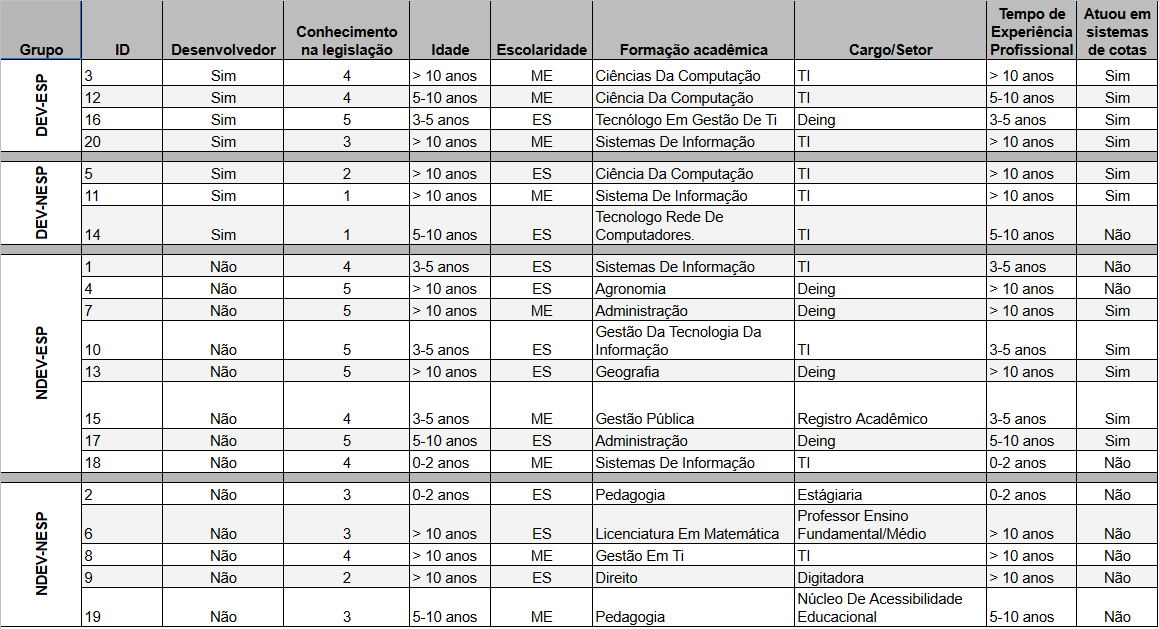
\includegraphics[width=1.5\textwidth]{chapters/analise/imagens/perfilusuarios.png}}

\par\medskip\textbf{Fonte:} Elaboração do autor (2020). \par\medskip

\end{figure}

\end{landscape}

\section{Resultados obtidos com o exercício}
\label{sec:analiseexercicio}




\section{Resultados obtidos com a aplicação do questionário}
\label{sec:questionarioexercicio}




\section{Resultados objetivos com a aplicação da API}
\label{sec:avaliacaoapi}


\section{Mudanças resultantes da avaliação}
\label{sec:mudanasresultantes}